\documentclass[10pt]{article}
\usepackage[utf8]{inputenc}
\usepackage[T1]{fontenc}
\usepackage{amsmath}
\usepackage{amsfonts}
\usepackage{amssymb}
\usepackage{mhchem}
\usepackage{stmaryrd}
\usepackage{graphicx}
\usepackage[export]{adjustbox}
\graphicspath{ {./images/} }

\title{Lesson 7: }

\author{}
\date{}


\begin{document}
\maketitle
\section{Disinfection}
\section{Objective}
In this lesson we will answer the following questions:

\begin{itemize}
  \item What disinfection requirements must be met in treating drinking water?

  \item How does chlorination fit into the water treatment process?

  \item How does chlorination work chemically?

  \item What factors influence the efficiency of chlorination?

  \item What equipment is used for chlorination?

  \item What other methods can be used to disinfect water?

\end{itemize}
\section{Reading Assignment}
Along with the online lesson, read Chapter 7: Disinfection, in your textbook Operation of Water Treatment Plants Volume I .

\section{Lecture}
\section{Introduction}
\section{What is Disinfection?}
Before water treatment became common, waterborne diseases could spread quickly through a population, killing or harming hundreds of people. The table below shows some common, water-transmitted diseases as well as the organisms (pathogens) which cause each disease. More information on water-borne pathogens can be found in ENV 108.

\begin{tabular}{|c||l|}
\hline
\multicolumn{1}{|c|}{Pathogen} & \multicolumn{1}{c|}{Disease Caused} \\
\hline
Bacteria: &  \\
\hline\hline
Anthrax & anthrax \\
\hline\hline
Escherichia coli & E. coli infection \\
\hline\hline
Myobacterium & tuberculosis \\
tuberculosis &  \\
\hline\hline
Salmonella & salmonellosis, \\
paratyphoid &  \\
\hline\hline
Vibrio cholerae & cholera \\
\hline\hline
Viruses: &  \\
\hline\hline
Hepatitis Virus & Hepatitis A \\
\hline\hline
Polio Virus & polio \\
\hline\hline
Parasites: &  \\
\hline\hline
Cryptosporidium & cryptosporidiosis \\
\hline\hline
Giardia lamblia & giardiasis \\
\hline\hline
\end{tabular}

The primary goal of water treatment is to ensure that the water is safe to drink and does not contain any disease-causing microorganisms. The best way to ensure pathogen-free drinking water is to make sure that the pathogens never enter the water in the first place. However, this may be a difficult matter in a surface water supply which is fed by a large watershed. Most treatments plants choose to remove or kill pathogens in water rather than to ensure that the entire watershed is free of pathogens.

Pathogens can be removed from water through physical or chemical processes. You may remember that some previously discussed treatment processes, notably sedimentation and filtration, can remove a large percentage of bacteria and other microorganisms from the water by physical means. Storage can also kill a portion of the disease-causing bacteria in water. This lesson will be concerned with disinfection, which is the process of selectively destroying or inactivating pathogenic organisms in water, usually by chemical means. Disinfection is different from sterilization, which is the complete destruction of all organisms found in water and which is usually expensive and unnecessary. Disinfection is a required part of the water treatment process while sterilization is not.

Disinfection refers to an operation in which we hope to inactivate the microorganisms in water that can cause an infection or disease. These organisms are collectively referred to as pathogens and include many species of bacteria, fungus, protozoa, worms, viruses, etc. Fortunately, not all microbes in water are of concern, so disinfection operations are not designed to actually sterilize the water, or kill all the microbes. It would not be economically feasible or practical to sterilize the large volumes of drinking water that we require each day. Instead, the government has provided guidelines for disinfection operations, based on disinfectant concentration and contact time, that should provide for sufficient inactivation of the more common and resistant microbes. In this way, we should be inactivating the multitude of pathogens that are less resistant. The presence or absence of coliform bacteria is generally tested at a water plant to determine if the water is biologically safe for consumption. Coliforms are therefore often referred to as indicator organisms.

We would also hope that the chemicals used for disinfection (the disinfectants) can minimize or eliminate the problems caused by nuisance organisms. For example, organisms can grow in the plant or in pipelines that might harbor pathogens and/or cause odors, tastes, and turbidity. Thus, disinfectants are used to maintain and clean plant facilities (e.g., to reduce biofilms) and to maintain a residual in distribution lines. Use of disinfectants in this manner is referred to as secondary disinfection, as opposed to primary disinfection which focuses on the in-plant inactivation of pathogens. Disinfection practices are indeed important because they represent the last line of defense against biological contaminants at a waterworks.

Among the more commonly used disinfectants are chlorine, chloramines, chlorine dioxide, ozone, potassium permanganate, and ultraviolet light.

Disinfectants typically kill pathogens in one of five ways:

\begin{enumerate}
  \item The disinfectant damages the cell wall.

  \item The disinfectant alters the pathogen's ability to pass food and waste through the cell membrane.

  \item The disinfectant alters the cell protoplasm.

  \item The disinfectant inhibits cellular conversion of food to energy.

  \item The disinfectant inhibits reproduciton.

\end{enumerate}
\section{Coliforms}
Coliform bacteria are often the only microbes routinely tested at a water treatment plant to assess the biological safety of a water. In larger plants with more resources, other microbes might be tested, as well. There are two basic groups of coliforms; those that are found in soil and those that are present in the manure, or feces, of warm-blooded animals, including humans. We do not want to see either bacterial group in our drinking water. The presence of the soil group could mean there is a break in the water line, and the presence of the fecal group could mean sewage has entered the water supply. Typically, operators will look for the presence or absence of total coliforms, and then, if the results are positive, they will do an additional test to figure out if the coliforms are soil or fecal types. The common fecal type tested is Escherichia coli or E. coli.

\section{Chlorination}
In the U.S., the disinfectant of choice has been chlorine. In general, chlorination is effective, relatively inexpensive, and provides effective levels of disinfectant residual for safe distribution. Applied as a gas (elemental chlorine, $\mathrm{Cl}_{2}$ ), liquid (sodium hypochlorite), or solid (calcium hypochlorite), each of these forms has advantages and disadvantages.

The most cost-effective and efficient, in terms of available chlorine, is gaseous chlorine. One volume of liquid chlorine under pressure will yield roughly 450 volumes of gas. Large treatment plants commonly use this method, creating gas from liquid chlorine stored on-site in high-pressure, high-strength steel cylinders. Gaseous chlorination is also the most inherently dangerous method - chlorine gas is lethal at concentrations as low as $0.1 \%$ air by volume. In nonlethal concentrations, it irritates the eyes, nasal membranes, and respiratory tract. Safety requirements for gaseous chlorine are extensive.

Because of the stiff safety requirements, and because it is easier to use and less toxic than gaseous chlorine, sodium hypochlorite (the form of chlorine in laundry bleach) is the most common disinfectant in smaller systems. Usually diluted with water before being applied as a disinfectant, sodium hypochlorite provides 5 to $15 \%$ available chlorine. Sodium hypochlorite must be handled and stored with care, and its corrosiveness means it must be kept isolated from vulnerable machinery. Sodium hypochlorite solution costs more per pound of available chlorine, and provides lower levels of protection against pathogens than chlorine gas. Because of regulatory pressures, some large water treatment facilities are converting to sodium hypochlorite disinfection.

Calcium hypochlorite (a white solid available as tablets, powder, or in granular form) contains $65 \%$ available chlorine. Packaged calcium hypochlorite is stable, though it readily absorbs moisture from the air, reacting with it to form chlorine gas. It is also corrosive, strong smelling, and requires proper handling. When in contact with organic materials, including wood, cloth, and petroleum products, chemical reactions can cause fire or explosion. Though some forms of chlorine are safer to handle than others, using any form of chlorine for disinfection requires special care and skill from the operator.

Chlorine, whether elemental chlorine, sodium hypochlorite, or calcium hypochlorite, may be added to the incoming flow (prechlorination) or, instead, added right before filtration. When used in prechlorination, chlorine works to help oxidize inorganics, and halts the biological action that occurs in the accumulations on the bottoms of clarifiers, preventing dangerous gaseous buildups. Chlorination prior to filtration keeps algae from growing and bacterial populations from developing in and on the filter itself.

Common terms used in chlorination include the following:

Chlorine Dose - the amount of chlorine added to the system. It can be determined by adding the desired residual for the finished water to the chlorine demand of the untreated water. Dosage can be either milligrams per liter (mg/L) or pounds per day (lb/day).

Chlorine Dose $(\mathrm{mg} / \mathrm{L})=$ Chlorine Demand $+$ Chlorine Residual

Chlorine Demand - the amount of chlorine used by iron, manganese, turbidity, algae, and microorganisms in the water. Because the reaction between chlorine and microorganisms is not instantaneous, demand is relative to time. For instance, the demand 5 minutes after applying chlorine will be less than the demand after 20 minutes. Demand, like dosage, is expressed in $\mathrm{mg} / \mathrm{L}$. The chlorine demand is as follows:

Chlorine Demand $=$ Chlorine Dose $-$ Chlorine Residual

Chlorine Residual - the amount of chlorine (determined by testing) remaining after the demand is satisfied. Residual, like demand, is based on time. The longer the time after dosage, the lower the residual will be, until all of the demand has been satisfied. Residual, like dosage and demand, is expressed in $\mathrm{mg} / \mathrm{L}$. The presence of a free residual of at least $0.2$ to $0.4 \mathrm{ppm}$ usually provides a high degree of assurance that the disinfection of the water is complete. Combined residual is the result of combining free chlorine with nitrogen compounds. Combined residuals are also referred to as chloramines. Total chlorine residual is the mathematical combination of free and combined residuals. Total residual can be determined directly with standard chlorine residual test kits.

The chlorine dosage feed rate can be determined with the following formula:

Chlorine feed rate $(\mathrm{lb} /$ day $)=$ Chlorine $(\mathrm{mg} / \mathrm{L}) \times$ Flow $(\mathrm{MGD}) \times 8.34 \mathrm{lb} / \mathrm{gal}$

\section{Example 1:}
Determine the chlorinator setting (lb/day) required to treat a flow of $4 \mathrm{MGD}$ with a chlorine dose of $5 \mathrm{mg} / \mathrm{L}$.

Chlorine feed rate $(\mathrm{lb} /$ day $)=$ Chlorine $(\mathrm{mg} / \mathrm{L}) \times$ Flow $(\mathrm{MGD}) \times 8.34 \mathrm{lb} / \mathrm{gal}$

Chlorine feed rate $(\mathrm{lb} /$ day $)=5 \mathrm{mg} / \mathrm{L} \times 4 \mathrm{MGD} \times 8.34 \mathrm{lb} / \mathrm{gal}$

Chlorine feed rate $(\mathrm{lb} /$ day $)=167 \mathrm{lb} /$ day

\section{Example 2 :}
A pipeline that is 12 inches in diameter and $1400 \mathrm{ft}$ long is to be treated with a chlorine dose of $48 \mathrm{mg} / \mathrm{L}$. How many lb of chlorine will this require?

First determine the gallon volume of the pipeline:

Volume $(\mathrm{gal})=0.785 \times \mathrm{D}^{2} \times$ length $(\mathrm{ft}) \times 7.48 \mathrm{gal} / \mathrm{cu} \mathrm{ft}$

Volume $(\mathrm{gal})=0.785 \times(1 \mathrm{ft})^{2} \times 1400 \mathrm{ft} \times 7.48 \mathrm{gal} / \mathrm{cu} \mathrm{ft}$ Volume $(\mathrm{gal})=8221 \mathrm{gal}$

Next calculate the amount of chlorine required:

Chlorine feed rate $(\mathrm{lb} /$ day $)=$ Chlorine $(\mathrm{mg} / \mathrm{L})$ x Flow $($ MGD) $\times 8.34 \mathrm{lb} / \mathrm{gal}$

Chlorine feed rate $(\mathrm{lb} /$ day $)=48 \mathrm{mg} / \mathrm{L} \times 0.008221 \mathrm{MGD} \times 8.34 \mathrm{lb} / \mathrm{gal}$

Chlorine feed rate $(\mathrm{lb} /$ day $)=3.3 \mathrm{lb}$

\section{Example 3:}
A water sample is tested and found to have a chlorine demand of $1.7 \mathrm{mg} / \mathrm{L}$. If the desired chlorine residual is $0.9 \mathrm{mg} / \mathrm{L}$, what is the desired chlorine dose (in $\mathrm{mg} / \mathrm{L}$ )?

Chlorine Dose $(\mathrm{mg} / \mathrm{L})=$ Chlorine Demand $+$ Chlorine Residual

Chlorine Dose $(\mathrm{mg} / \mathrm{L})=1.7 \mathrm{mg} / \mathrm{L}+0.9 \mathrm{mg} / \mathrm{L}$

Chlorine $\operatorname{Dose}(\mathrm{mg} / \mathrm{L})=2.6 \mathrm{mg} / \mathrm{L}$

\section{Example 4:}
The chlorine dosage for water is $2.7 \mathrm{mg} / \mathrm{L}$. If the chlorine residual after a 30-minute contact time is found to be $0.7 \mathrm{mg} / \mathrm{L}$, what is the chlorine demand (in $\mathrm{mg} / \mathrm{L}$ )?

Chlorine Demand $=$ Chlorine Dose $-$ Chlorine Residual

Chlorine Demand $=2.7 \mathrm{mg} / \mathrm{L}-0.7 \mathrm{mg} / \mathrm{L}$

Chlorine Demand $=2.0 \mathrm{mg} / \mathrm{L}$

\section{Example 5:}
What should the chlorinator seting be (lb/day) to treat a flow of $2.35 \mathrm{MGD}$ if the chlorine demand is $3.2 \mathrm{mg} / \mathrm{L}$ and a chlorine residual of $0.9 \mathrm{mg} / \mathrm{L}$ is desired?

First, determine the chlorine dosage (in $\mathrm{mg} / \mathrm{L}$ ):

Chlorine Dose $(\mathrm{mg} / \mathrm{L})=$ Chlorine Demand $+$ Chlorine Residual

Chlorine Dose $(\mathrm{mg} / \mathrm{L})=3.2 \mathrm{mg} / \mathrm{L}+0.9 \mathrm{mg} / \mathrm{L}$

Chlorine Dose $(\mathrm{mg} / \mathrm{L})=4.1 \mathrm{mg} / \mathrm{L}$

Next calculate the chlorine dosage (feed rate) in $\mathrm{lb} /$ day:

Chlorine feed rate $(\mathrm{lb} /$ day $)=$ Chlorine $(\mathrm{mg} / \mathrm{L}) \times$ Flow $(\mathrm{MGD}) \times 8.34 \mathrm{lb} / \mathrm{gal}$

Chlorine feed rate $(\mathrm{lb} /$ day $)=4.1 \mathrm{mg} / \mathrm{L} \times 2.35 \mathrm{MGD} \times 8.34 \mathrm{lb} / \mathrm{gal}$

Chlorine feed rate $(\mathrm{lb} /$ day $)=80.4 \mathrm{lb} /$ day

\section{Breakpoint Chlorination}
To produce a free chlorine residual, enough chlorine must be added to the water to produce what is referred to as breakpoint chlorination (i.e., the point at which near complete oxidation of nitrogen compounds is reached; any residual beyond breakpoint is mostly free chlorine). When chlorine is added to natural waters, the chlorine begins combining with and oxidizing the chemicals in the water before it begins disinfecting. Although residual chlorine will be detectable in the water, the chlorine will be in the combined form with a weak disinfecting power. As you can see in the image below, adding more chlorine to the water at the point actually decreases the chlorine residual as the additional chlorine destroys the combined chlorine compounds.

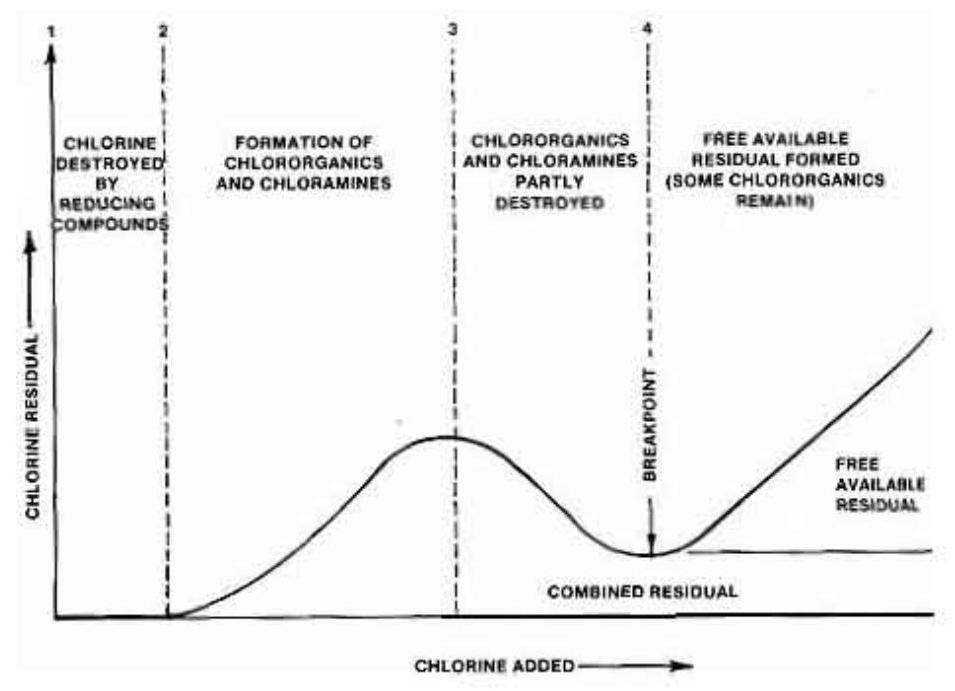
\includegraphics[max width=\textwidth]{2022_10_14_eba0aec33b37be0fbdf2g-05}

At this stage, water may have a strong swimming pool or medicinal taste and odor. To avoid this taste and odor, add still more chlorine to produce a free residual chlorine. Free chlorine has the highest disinfecting power. The point at which most of the combined chlorine compounds have been destroyed and the free chlorine starts to form is the breakpoint. The actual chlorine breakpoint of water can only be determined by experimentation. To calculate the actual increase in chlorine residual that would result from an increase in chlorine dose, use the following equaiton:

Increase in chlorine dose $(\mathrm{lb} /$ day $)=$ expected increase $(\mathrm{mg} / \mathrm{L}) \times$ flow $(\mathrm{MGD}) \times 8.34 \mathrm{lb} / \mathrm{gal}$

The actual increase in residual is simply a comparison of new and old residual data.

\section{Example 1:}
A chlorinator setting is increased by $2 \mathrm{lb} /$ day. The chlorine residual before the increased dosage was $0.2 \mathrm{mg} / \mathrm{L}$. After the increased chlorine dose, the chlorine residual was $0.5 \mathrm{mg} / \mathrm{L}$. The average flow rate being chlorinated is $1.25 \mathrm{MGD}$. Is the water being chlorinated beyond the breakpoint?

First calculate the expected increase in chlorine residual:

Chlorine feed rate $(\mathrm{lb} /$ day $)=$ Chlorine $(\mathrm{mg} / \mathrm{L})$ x Flow $(\mathrm{MGD}) \times 8.34 \mathrm{lb} / \mathrm{gal}$

$2 \mathrm{lb} /$ day $=\times \mathrm{mg} / \mathrm{L} \times 1.25 \mathrm{MGD} \times 8.34 \mathrm{lb} / \mathrm{gal}$

$x=2 /(1.25 \times 8.34)$

$\mathrm{x}=0.19 \mathrm{mg} / \mathrm{L}$

Actual increase in residual is:

$0.5 \mathrm{mg} / \mathrm{L}-0.19 \mathrm{mg} / \mathrm{L}=0.31 \mathrm{mg} / \mathrm{L}$

\section{Example 2:}
A chlorinator setting of $18 \mathrm{lb}$ chlorine per 24 hours result in a chlorine residual of $0.3 \mathrm{mg} / \mathrm{L}$. The chlorinator setting is increased to $22 \mathrm{lb}$ per 24 hours. The chlorine residual increased to $0.4 \mathrm{mg} / \mathrm{L}$ at this new dosage rate. The average flow being treated is $1.4 \mathrm{MGD}$. On the basis of these data, is the water being chlorinated past the breakpoint?

First calculate the expected increase in chlorine residual:

Chlorine feed rate $(\mathrm{lb} /$ day $)=$ Chlorine $(\mathrm{mg} / \mathrm{L}) \times$ Flow $(\mathrm{MGD}) \times 8.34 \mathrm{lb} / \mathrm{gal}$

$4 \mathrm{lb} /$ day $=\mathrm{x} \mathrm{mg} / \mathrm{L} \times 1.4 \mathrm{MGD} \times 8.34 \mathrm{lb} / \mathrm{gal}$

$\mathrm{x}=4 /(1.4 \times 8.34)$

$\mathrm{x}=0.34 \mathrm{mg} / \mathrm{L}$

Next calculate the actual increase in residual:

$0.4 \mathrm{mg} / \mathrm{L}-0.3 \mathrm{mg} / \mathrm{L}=0.1 \mathrm{mg} / \mathrm{L}$

\section{Contact Time}
Contact time is just as important as the chlorine residual in determining the efficiency of chlorination. Contact time is the amount of time which the chlorine has to react with the microorganisms in the water, which will equal the time between the moment when chlorine is added to the water and the moment when that water is used by the customer. The longer the contact time, the more efficient the disinfection process is. When using chlorine for disinfection a minimum contact time of 30 minutes is required for adequate disinfection.

An operator measures the amount of contact time available at the plant before the water goes out to the public to ensure that $99.9 \%$ of giardia lamblia is either removed with filtration or inactivated with chlorine before the water gets to the public. The operator compares the contact time at the plant to the CT tables provided by the EPA. As long as the contact time the operator measures at the plant is greater than that required by the EPA, the water passes the disinfection portion of the treatment process.

The "baffling efficiency" of a tank is used to determine chlorine contact time in the tank. If the water used to calculate disinfection contact time moves through a storage tank, pressure tank, or pipes too quickly, the situation is called "shortcircuiting". Some vessels provide better contact time than others do. Water systems can modify reservoirs to improve the baffling efficiency. In some cases little or no baffling efficiency can be awarded. Pipes with a length to width ratio of 150 or more typically have a baffling efficiency of 100 percent.

In summary, to calculate CT you must know:

\begin{enumerate}
  \item The contact time (T) for each water system component between the chlorine injection point and where free chlorine is measured before the first customer.

  \item The volume and baffling efficiency of each component.

  \item The peak flow through each component.

  \item The free chlorine residual measured downstream of all the components and upstream of the first customer.

\end{enumerate}
When calculating Contact Time, use the lowest volume of water in the tank under non-emergency/normal operating conditions.

The following steps have been set up to help operators determine contact time.

Step 1: Determine the time available in the basin at peak flow. Multiply the basin volume by the baffling factor and divide by the Peak Hourly Flow to determine the Time portion of the contact time equation.
$$
\text { Time }(\min )=\frac{\text { Basin Volume }(\text { gal }) \mathrm{x} \text { baffling factor }}{\text { Peak Hourly Flow }(\mathrm{gpm})}
$$
Step 2: Determine the contact time available at peak flow. Multiply the Time by your chlorine concentration at peak hourly flow. This is the Contact Time you have available.

Available Contact Time $(\min \mathrm{mg} / \mathrm{L})=$ Time $(\mathrm{min}) \times$ Chlorine concentration $(\mathrm{mg} / \mathrm{L})$

Step 3: Find the required Contact Time (CT) from the tables at peak flow. Determine the CT required by the EPA. You need to do this by looking up the CT from the CT tables provided using your $\mathrm{pH}$, temperature and chlorine concentration.

Step 4: Does your water system meet CT requirements?

Compute the inactivation ratio by dividing the actual contact time by required contact time. If the rateo is greater than 1 , then your water system met its contact time requirements. If you cannot meet contact time, you can either increase your storage volume or increase your disinfectant residual.

Inactivation Raio $=\frac{\text { Actual Contact Time }}{\text { Required Contact Time }}$

\section{Example:}
Your campground has a 5,000 gallon steel tank. An engineer has determined that the baffling factor for the tank is $0.3$. The flow of water through the system is determined to be 15 gallons per minute at maximum flow conditions. The pH is $7.0$ and the temperature is 10 Celsius. Determine whether or not your campground meets contact time requirements at $1.5 \mathrm{mg} / \mathrm{L}$ chlorine.

Step 1:
$$
\begin{aligned}
&\text { Time }(\min )=\frac{5,000 \mathrm{gal} \times 0.3}{15 \mathrm{gpm}} \\
&\text { Time }(\min )=100
\end{aligned}
$$
Step 2: Available Contact Time ( $\min \mathrm{mg} / \mathrm{L})=$ Time $(\mathrm{min}) \times$ Chlorine concentration $(\mathrm{mg} / \mathrm{L})$

Available Contact Time $(\min \mathrm{mg} / \mathrm{L})=100 \mathrm{~min} \times 1.5 \mathrm{mg} / \mathrm{L}$

Available Contact Time $(\min \mathrm{mg} / \mathrm{L})=150$

Step 3: Look up the contact time that you need to achieve from the following table. TABLE E-3

CT YALUES FOR INACTIVATION OF GIARDIA CYSTS BY FREE CHLORNE

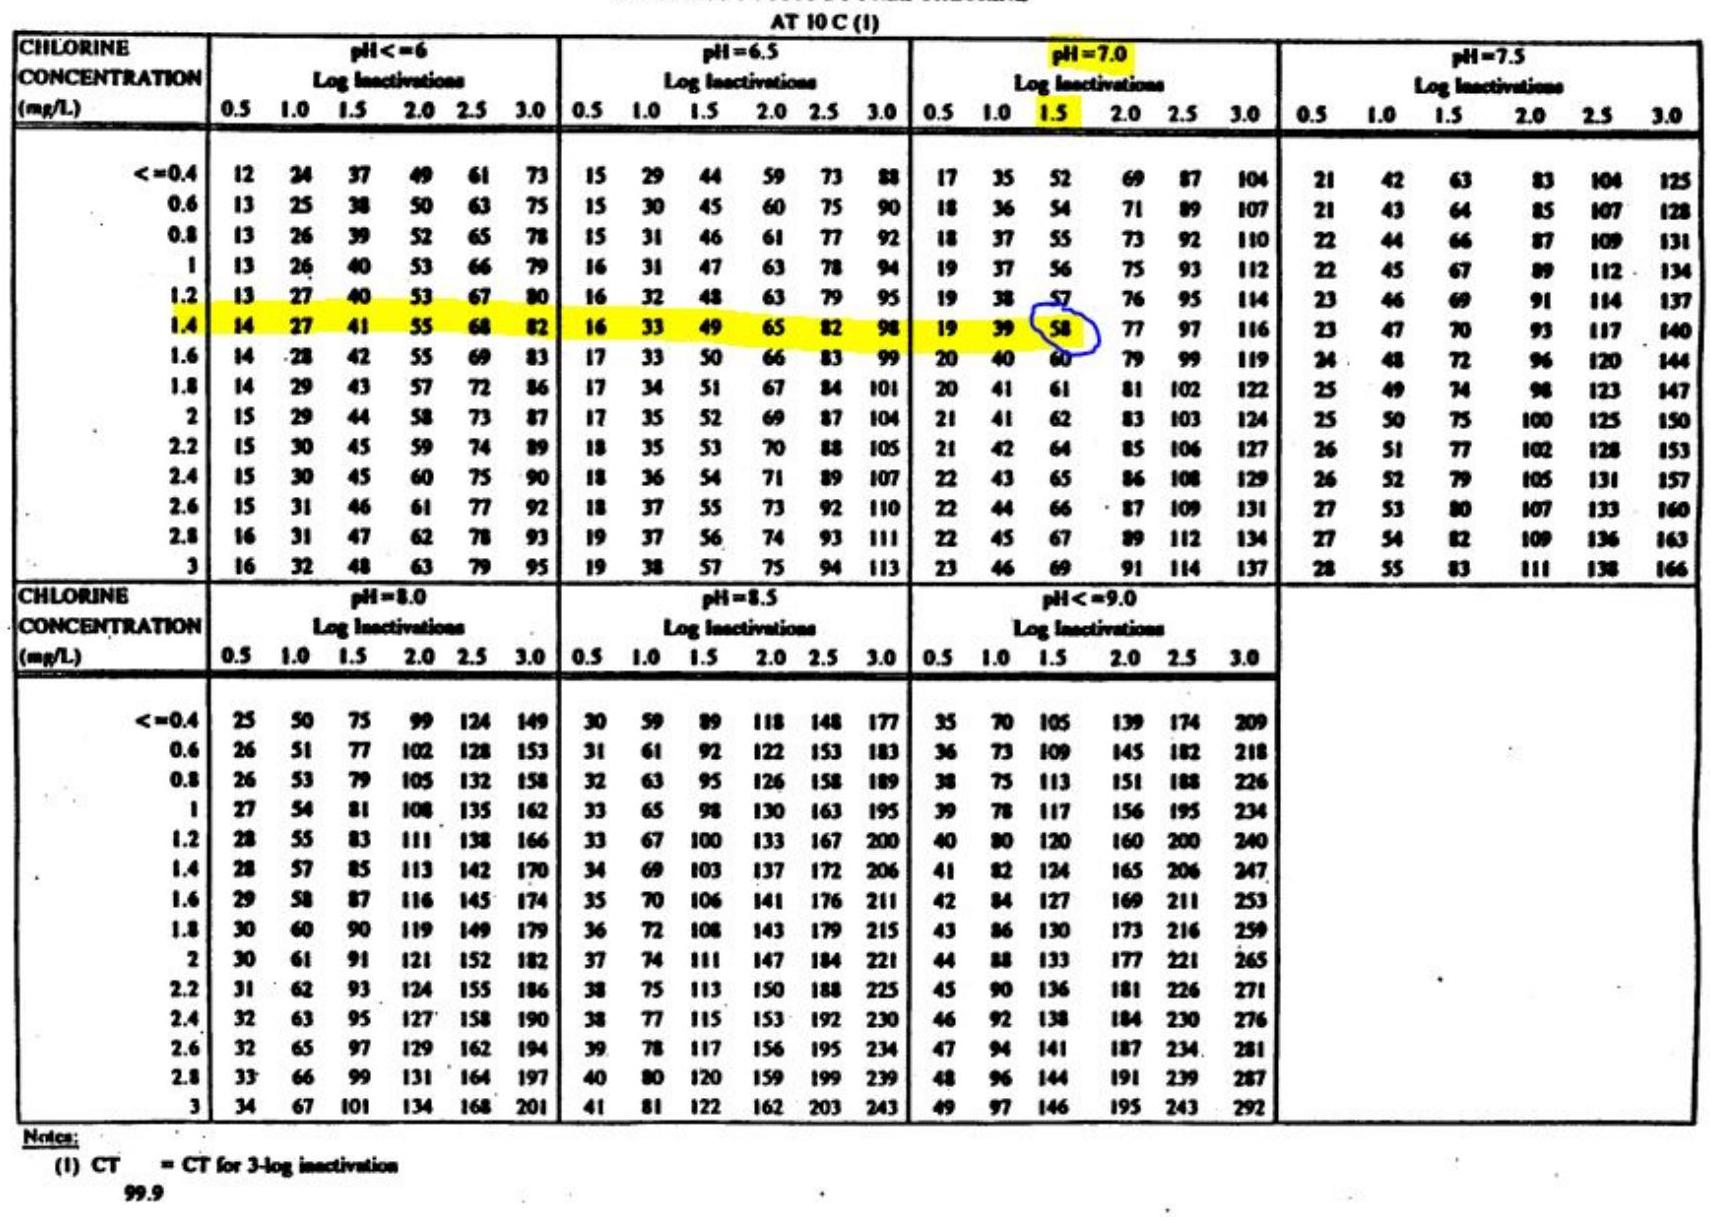
\includegraphics[max width=\textwidth]{2022_10_14_eba0aec33b37be0fbdf2g-08}

You will notice under the Chlorine Concentration $(\mathrm{mg} / \mathrm{L})$ column, $1.5 \mathrm{mg} / \mathrm{L}$ is not listed, so use the next lowest chlorine residual, $1.4 \mathrm{mg} / \mathrm{L}$. Look at the table at $1.4 \mathrm{mg} / \mathrm{L}$ and go across to the $\mathrm{pH}=7.0$. The CT required for compliance, from the table, is $58 \mathrm{~min} \mathrm{mg} / \mathrm{L}$.

Step 4: Is the inactivation ratio greater than 1 ? Divide 150 by 58 to get $2.6$. Since $2.6$ is greater than 1 your system did meet the contact time requirements.
$$
\begin{aligned}
&\text { Inactivation Raio }=\frac{150}{58} \\
&\text { Inactivation Raio }=2.6
\end{aligned}
$$
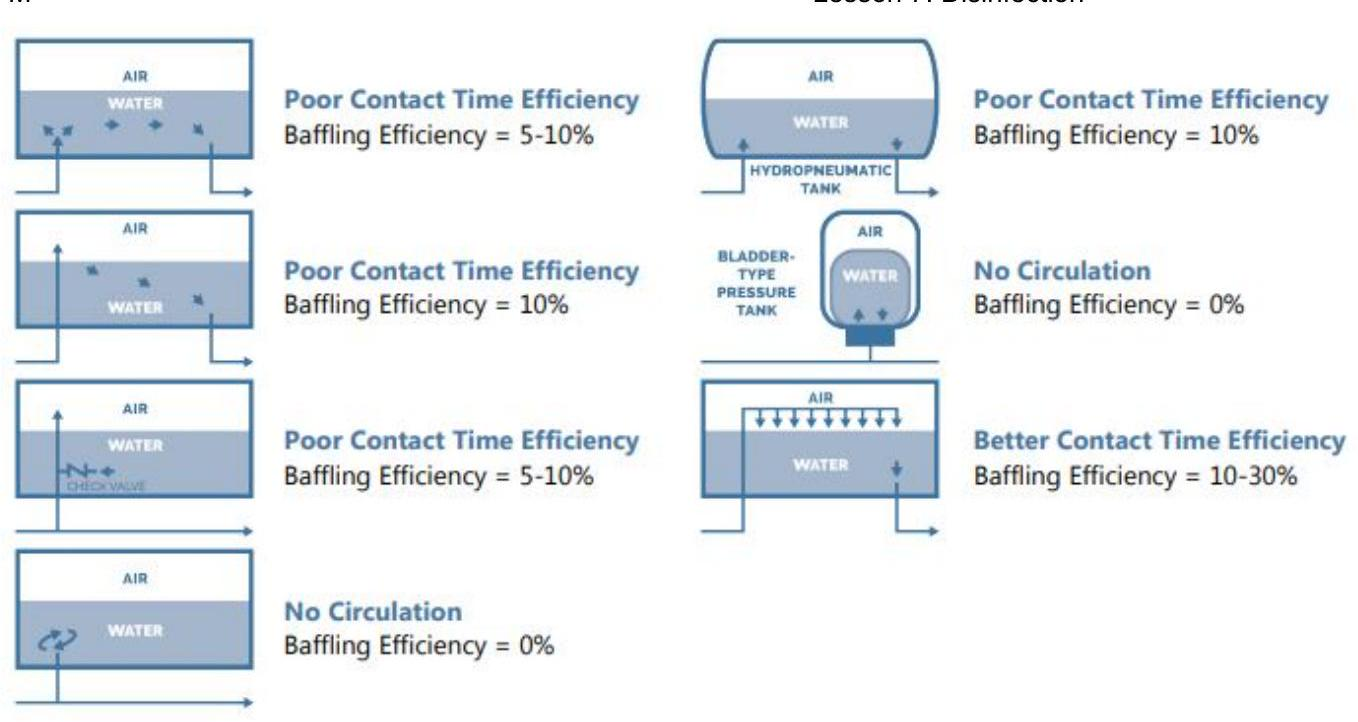
\includegraphics[max width=\textwidth]{2022_10_14_eba0aec33b37be0fbdf2g-09}

\section{Prechlorination and Postchlorination}
Like several other water treatment processes, chlorination can be used as a pretreatment process (prechlorination) or as part of the primary treatment of water (postchlorination). Treatment usually involves either postchlorination only or a combination of prechlorination and postchlorination.

Prechlorination is the act of adding chlorine to the raw water. The residual chlorine is useful in several stages of the treatment process - aiding in coagulation, controlling algae problems in basins, reducing odor problems, and controlling mudball formation. In addition, the chlorine has a much longer contact time when added at the beginning of the treatment process, so prechlorination increases safety in disinfecting heavily contaminated water.

Postchlorination is the application of chlorine after water has been treated but before the water reaches the distribution system. At this stage, chlorination is meant to kill pathogens and to provide a chlorine residual in the distribution system. Postchlorination is nearly always part of the treatment process, either used in combination with prechlorination or used as the sole disinfection process.

Until the middle of the 1970 s, water treatment plants typically used both prechlorination and postchlorination. However, the longer contact time provided by prechlorination allows the chlorine to react with the organics in the water and produce carcinogenic substances known as trihalomethanes. As a result of concerns over trihalomethanes, prechlorination has become much less common in the United States. Currently, prechlorination is only used in plants where trihalomethane formation is not a problem.

\section{Location in the Treatment Process}
During prechlorination, chlorine is usually added to raw water after screening and before flash mixing. Postchlorination, in contrast, is often the last stage in the treatment process. After flowing through the filter, water is chlorinated and then pumped to the clearwell to allow a sufficient contact time for the chlorine to act. From the clearwell, the water may be pumped into a large, outdoor storage tank such as the one shown below. Finally, the water is released to the customer.

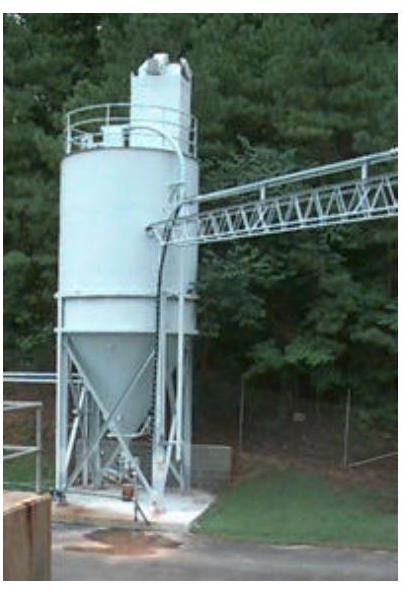
\includegraphics[max width=\textwidth]{2022_10_14_eba0aec33b37be0fbdf2g-10}

Photo Credit: Virginia Department of Health

\section{Factors Influencing Chlorination}
The efficiency of disinfection operations can be complex and is dependent upon several factors, including the chemistry of the disinfectant and the nature of the pathogen. However, in general, one would expect to see the following trends:

\begin{itemize}
  \item $\mathrm{pH}$ - improved disinfection as $\mathrm{pH}$ decreases.
\end{itemize}
Effectiveness of chlorine is $\mathrm{pH}$ dependent. The lower the $\mathrm{pH}$, the more effective the free-residual chlorine, and vice versa. Both hypochlorous acid and hypochlorite ions are called free-residual chlorine. The amount of hypochlorous acid, the principal disinfectant, decreases at above $\mathrm{pH} 7.5$ as it ionizes into hypochlorite ions.

\begin{itemize}
  \item Temperature - improved disinfection as temperature increases.
\end{itemize}
Effectiveness of chlorine varies directly with the temperature. The higher the temperature, the quicker the disinfection and shorter is the required contact time.

\begin{itemize}
  \item Disinfectant concentration - improved disinfection as concentration increases.
\end{itemize}
The higher the concentration, the more effective is the disinfectant. Normally, $0.5$ to 1 ppm free-residual chlorine will effectively disinfect the water. According to the Safe Drinking Water Act, the maximum allowed chlorine residual in the distribution system is $4 \mathrm{mg} / \mathrm{L}$ and the minimum required is $0.2 \mathrm{mg} / \mathrm{L}$.

\begin{itemize}
  \item Time of contact - improved disinfection as time increases.
\end{itemize}
Chlorine requires a certain amount of contact time at different temperatures to react with microorganisms. The longer the contact time, the more effective is the disinfection.

\begin{itemize}
  \item Turbidity - improved disinfection as turbidity decreases
\end{itemize}
Thus, to improve the efficiency of disinfection, we might consider reducing $\mathrm{pH}$, depending on disinfectant being used, increasing the amount of disinfectant, changing the point where disinfectant is added to increase contact time, and removing more turbidity (solids). We might also be able to consider changing temperature if we can withdraw water at different levels in a reservoir, but for the most part, we just have to deal with the water temperatures that naturally occur. Manipulation of these factors, of course, has to be balanced against costs and the possibility that we will also affect changes in DBP formation. It is difficult to generalize how all disinfection systems should be designed and operated, bu tthe EPA has established regulations and guidelines that are seemingly serving the public well. The CT concept is an example of the guidance that has been provided by the EPA.

\section{Chlorination Chemistry}
In water, chlorine reacts with various substances or impurities present (organic materials, sulfides, ferrous iron, and nitrites, for example). The presence of these materials creates a chlorine demand, a measure of the amount of chlorine needed to eliminate these impurities by combining with them. That amount of chlorine cannot disinfect; it is already chemically depleted.

Chlorine also combines readily with ammonia or other nitrogen compounds, forming chlorine compounds. These chlorine compounds have some disinfectant properties, and are called the combined available chlorine residual. Chlorine in this form acts as a disinfectant. The chemically unchanged chlorine remaining in the water after combined residual is formed is free available chlorine residual. Free chlorine is much more effective than combined chlorine in disinfection.

For successful chlorination, several factors must be addressed: concentration of free chlorine, contact time, temperature, pH, and turbidity. How effectively chlorine disinfects is directly related to contact time with the water, as well as the free available chlorine concentration. Lower chlorine concentrations require increased contact times. Lower pH levels also aid disinfection effectiveness. Chlorine disinfects more quickly at higher temperatures. Turbidity affects chlorine's effectiveness as well, as it does any disinfectant. Chlorine must contact organisms to kill them. High turbidity levels provide shelter for microorganisms, preventing efficient contact.

\section{Chlorination Equipment}
Chlorine is usually fed continuously to the influent. Probably the safest and most commonly used chlorine feed devices are all-vacuum chlorinators. They are installed directly on the chlorine cylinder. The chlorinator ensures that gaseous chlorine under a partial vacuum in the line is carried to the point of application. Typically, the vacuum is formed by water flowing through the ejector unit at high velocity. Usual application methods for hypochlorites involve adding the chemical in liquid form using positive displacement pumps. These deliver a specific amount of liquid on each stroke of a piston or flexible diaphragm.

\section{Chlorination By-Products}
Although using chlorine for disinfection is common, efficient, effective, and relatively inexpensive, recent studies show risks related to the potential formulation of chlorine by-products. Organic compounds, including decaying vegetation, combine with chlorine chemically, forming trihalomethanes (THMs). Chloroform (one of the THMs) is a suspected carcinogen, and other common trihalomethanes are chemically similar to chloroform, and raise concerns.

While many public utilities are exploring alternative methods of disinfection, others use approaches to reduce the possibility of chlorine by-product formation. Removing more of the organics before adding chlorine is a productive approach, as is simply changing the point in the treatment process where chlorine is added. These two approaches are generally accomplished by not chlorinating the raw water before filtration. Sometimes aeration or activated carbon adsorption is used to remove more organic materials. Reducing chlorine use to achieve a safe degree of disinfection with less chemical addition is also a possibility.

\section{Chlorine Health and Safety}
Chlorine is a very toxic gas, even in small concentrations in air. OSHA allows less than 1 ppm of chlorine in the air. The table below shows the physiological effects of various concentrations of chlorine by volume in the air.

\begin{tabular}{|l|l|}
\hline
Effects & Chlorine as ppm in Air \\
\hline
Least detectable by odor & below 3.5 \\
\hline
Produces throat irritation & 15 \\
\hline
Produces coughing & 30 \\
\hline
Dangerous for 30 minutes exposure & $40-60$ \\
\hline
Rapidly fatal & 1,000 \\
\hline
\end{tabular}

Observe the following precautions when dealing with chlorine:

\begin{itemize}
  \item Use a mask when entering a chlorine-containing atmosphere. Mask should be kept outside the chlorine room and checked regularly for leaks.

  \item Check chlorinator, lines, and cylinder valves regularly for leaks. Use ammonia fumes to test leaks. Ammonia and chlorine combine to produce white fumes of ammonium chloride, indicating a leak.

  \item Always store chlorine on the lowest floor because it is heavier than air and collects at the lowest level. Never stoop down when there is a chlorine smell in the room. Observe and meet all the OSHA requirements.

\end{itemize}
\section{Chloramines}
Chloramination is the use of chloramines for disinfection. Chloramines are produced by reacting ammonia with chlorine; they are slower and less effective than the free-residual chlorine $(\mathrm{HOCl})$. Therefore, they require a higher dose and longer contact time than the free-residual chlorine for the same degree of disinfection. Despite these drawbacks, they have been used successfully by a large number of utilities. Ammonia is used ahead of chlorine to prevent THM formation.

There are three species of chloramines: monochloramines, dichloramines, and trichloramines. Type of chloramine formation depends on the $\mathrm{pH}$ and chlorine-to-ammonia ratio. Above $\mathrm{pH} 8$ and ratio of chlorine to ammonia of 4 to 1 , monochloramine is the predominant species, which is preferred for disinfection because it is quite effective and less odorous. Below $\mathrm{pH} 8$ and the progression of chlorine to ammonia ratio, the species changes from monochloramines to dichloramines and from dichloramines to trichloramines.

Chloramination is more effective above $\mathrm{pH}$. Its effectiveness is comparable to hypochlorite ions. Its advantages are that there is no THM formation and it has a longer residual effect than chlorine. It is commonly used in postdisinfection for a longer residual effect in the distribution system.

Besides slow and weak disinfectants, chloramines include hemolytic anemia and cause problems with the use of dialysis machines; they are harmful to tropical fish. Due to these disadvantages, chloramines were not used by many utilities until the THM discovery in 1974.

\section{Chlorine Dioxide}
Chlorine dioxide, a yellow to red gas, is a very strong disinfectant produced by reacting sodium chlorite with chlorine or an acid. Unlike chlorine, its effectiveness is not affected by ammonia and $\mathrm{pH}$, and it does not produce THMs. Its effectiveness against Giardia and Cryptosporidium is reported as better than chlorine. It is very effective when followed by chlorine or chloramines. This sequential disinfection has a collaborating effect. A $1.5 \mathrm{mg} / \mathrm{L}$ chlorine dioxide dose alone gives only 90 percent reduction of these pathogens, whereas this dose followed by chlorine or chloramines gives about 99 percent reduction. However, chloramine and chlorine alone produce an insignificant effect. Apparently, chlorine dioxide weakens the pathogens and chlorine or chloramines destroy them.

Chlorine dioxide has disadvantages, however. It is an unstable compound that shortly reverts to chlorite; it is relatively expensive to generate; it is explosive at a concentration above 10 percent in the air; and it forms chlorites and chlorates. Being short lived, it is generated at the site and applied immediately. These disadvantages limit its application. By-products, chlorites and chlorates, cause an anemic condition in some individuals, resulting in a limit on the chlorine dioxide dose. Activated carbon, sulfur dioxide, sulfite, and ferrous compounds have been tested to neutralize these by-products. Out of these, the most practical and cost effective is the use of ferrous ions. About $3 \mathrm{mg} / \mathrm{L}$ ferrous ion concentration reduces chlorite by $1 \mathrm{mg} / \mathrm{L}$. Ferrous chloride is the commonly used source of ferrous ions.

\section{Alternative Methods of Disinfection}
The two most common alternative disinfection methods for water treatment are UV radiation and ozonation. Neither of these methods is an ideal solution for chlorine replacement, because of uncertainties and disadvantages with their use, i ncluding that they are not adequate for disinfection by themselves. While they do prevent the formation of THMs, both methods require secondary disinfection (usually chlorine) to maintain a residual during distribution.

\section{UV Radiation}
Ultraviolet (UV) radiation (electromagnetic radiation beyond blue at the end of the light spectrum, outside the visible light range) is a physical process, not a chemical process - a big advantage over both chlorine and ozone as disinfectants. It disinfects by inactivating bacteria and viruses. The genetic material in microorganisms absorbs UV energy (UV light has a higher energy level than visible light), interfering with reproduction and survival. Turbidity severely affects UV radiation's ability to inactivate microorganisms, however, providing shelter for microorganisms from contact with the light. Commonly, UV germicidal equipment consists of a series of submerged, low-pressure mercury lamps. Technological advances are making UV radiation a more viable disinfection alternative, in terms of both effectiveness and economics.

\section{Ozonation}
Ozone $\left(\mathrm{O}_{3}\right)$ used as disinfectant leaves no taste and odor in the treated water, is actually more effective than chlorine against some viruses and cysts, and is unaffected by $\mathrm{pH}$ or ammonia levels in the water. Ozone is a gas at normal temperatures and pressures, and disinfects by breaking up molecules in water. When ozone reacts with organic materials and inorganic compounds in water, an oxygen (instead of a chlorine) atom is added, resulting in an enviornmentally acceptable compound. Ozone's instability means that it cannot be stored and must be produced on-site, generating higher costs than chlorine disinfection. Since ozonation also provides no disinfection residual, those equipment, labor, and chemical costs must must also be factored in.

\section{Chlorination Equipment}
\section{Hypochlorinators}
The simplest method of continuous chlorination of systems less than $75 \mathrm{gpm}$ is by the use of a hypochlorinator.

Hypochlorinators are motor driven pumps which are used to added hypochlorite solutions to water. The pump pulls the hypochlorite solution out of a holding chamber and pumps it into the water to be treated. Where the pipe from the pump joins the pipe carrying the raw water, the Venturi effect creates a small vacuum and pulls the chlorine solution into the water.

\section{Hypochlorinator}
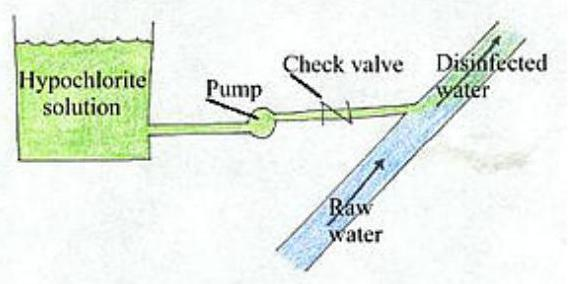
\includegraphics[max width=\textwidth]{2022_10_14_eba0aec33b37be0fbdf2g-13}

It is often necessary to increase or decrease the amount of chlorine added to the water as conditions change. Hypochlorinators allow you to adjust the amount of chlorine fed into the water in three ways. You can adjust the stroke length or machine speed by varying the pulley size. Both of these adjustments change the hypochlorinator feed rate - the speed at which the machine puts chlorine into the water. You can also adjust the amount of chlorine added by changing the strength of the hypochlorite solution.

\section{Chlorinators and Cylinders}
While hypochlorinators are usually used to perform continuous chlorination in smaller systems, chlorinators are more economical when the supply source is greater than $75 \mathrm{gpm}$ and may sometimes be used in smaller systems as well. Anticipated pumping periods and chlorine demand (based on the chlorine residual test) determine whether a hypochlorinator or chlorinator should be used in each situation.

Chlorinators are devices which introduce chlorine gas to water using liquid chlorine supplied in steel cylinders. The following sections will explain how the proper quantity of chlorine is delivered from the cylinder to the source water. But first we need to understand how the liquid chlorine is stored.

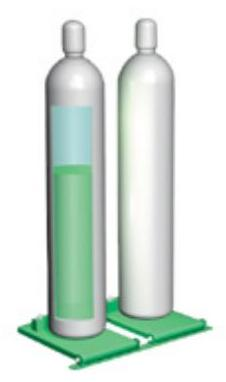
\includegraphics[max width=\textwidth]{2022_10_14_eba0aec33b37be0fbdf2g-14}

Chlorine cylinders

Liquid chlorine can be stored in 100 or 150 pound cylinders, ton containers, or 55 to 90 ton rail cars. In each case, the chlorine has been condensed into a liquid form, but expands back into a gas as it leaves the cylinder. Whenever a substance changes state from a liquid to a gaseous form, heat is required. The heat which is absorbed by the chlorine as it changes state in the cylinder comes from the surrounding air.

If chlorine is drawn off from a cylinder too quickly, the temperature of the air surrounding the tank will drop and will cause frosting and lower gas flow. To prevent frosting, the draw off rate should be no greater than 350 pounds of gas/day for a 100-150 pound cylinder. If greater feed rate are required, several tanks can be connected using a manifold, which is a pipe joining the cylinders together so that chlorine gas is drawn from several cylinders at once.

The only accurate way to determine the feed rate of chlorine from a cylinder is to weigh the cylinder over time. By subtracting the tare weight (the weight of an empty cylinder), the operator can determine how much chlorine gas remains in the cylinder so that empty cylinders can be replaced in a timely manner. If the cylinders are weighed over time, the feed rate of chlorine can be determined to ensure that the proper concentration of chlorine is being added to the water.

Whenever dealing with gaseous chlorine, safety is an important issue. Ammonia should be kept handy for checking for leaks and storage buildings should be well ventilated. If the operator must walk through an area with chlorine in the air, he or she should use a breathing apparatus. If no breathing apparatus is available, the operator should keep his head high since chlorine is $2.5$ times as heavy as air and will tend to sink to the ground.

\section{Vacuum Chlorinators}
The most typical kind of chlorinator, a vacuum chlorinator, is shown below:

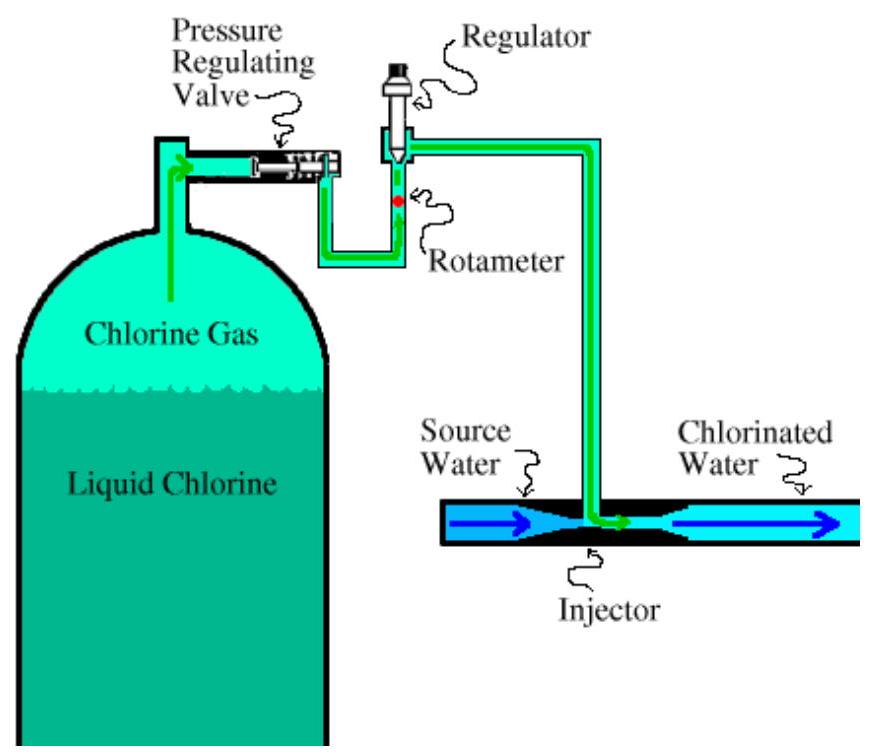
\includegraphics[max width=\textwidth]{2022_10_14_eba0aec33b37be0fbdf2g-14(1)}

In a vacuum chlorinator, chlorine gas is pulled from the cylinder into the source water by a vacuum. The vacuum is created by water flowing through the injector and creating a negative head. This negative head forces open the pressure regulating valve on the cylinder and allows chlorine gas to flow out of the cylinder and into the chlorinator.

Once the gas has entered the chlorinator, the chlorine feed rate is measured using an indicator known as a rotameter. Just beyond the rotameter, the chlorine gas flows past a regulating device (a V-notch plug or a valve) which is used to adjust the chlorine feed rate. Then the chlorine gas is pulled into the injector, also known as an ejector. The injector consists of a pipe filled with flowing water. The flowing water pulls chlorine into the water, both chlorinating the source water and creating a vacuum in the chlorine line which pulls more chlorine gas out of the cylinder. This type of chlorinator is also known as a solution feeder since the chlorine gas is dissolved into a small amount of source water, which is then piped into the main line of water to be chlorinated.

Chlorinators can be controlled manually (using the regulator) or with a controller. The most common type of controller is the flow proportional controller which automatically feeds chlorine based on the flow rate of the water.

Vacuum chlorinators are very safe since any break in the line with disrupt the vacuum and close the pressure regulating valve. As a result, chlorine leaks are very uncommon.

\section{Direct Feed Chlorinators}
In a few cases, direct feed chlorinators are used instead of vacuum chlorinators. In a direct feed chlorinator, the chlorine gas is under pressure and is pumped directly into the main flow of water. There, the chlorine is evenly dispersed into the water using a diffuser, like the one shown below.

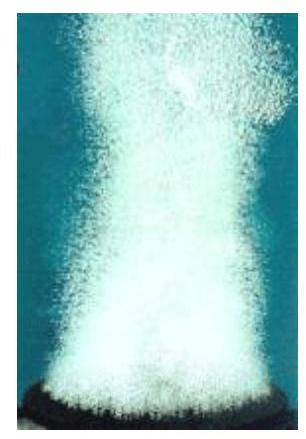
\includegraphics[max width=\textwidth]{2022_10_14_eba0aec33b37be0fbdf2g-15}

Since the chlorine is under pressure, a pressurized water supply is not needed for use with a direct feed chlorinator. However, the pressurized chlorine is prone to leakage, so safety issues limit direct feed chlorinators to small installations or for use as emergency equipment.

\section{Choosing a Disinfection Method}
Of the many disinfection methods, five have been used extensively in water treatment. The table below lists some of the factors which may influence the choice of treatment method in a new plant.

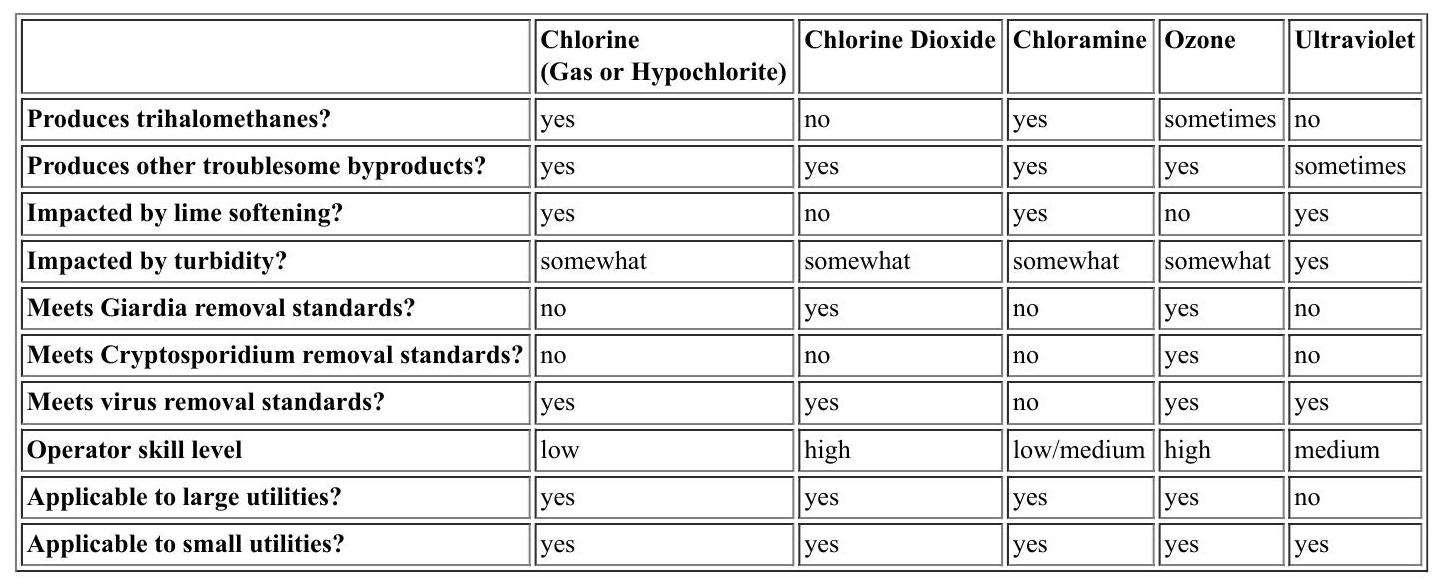
\includegraphics[max width=\textwidth]{2022_10_14_eba0aec33b37be0fbdf2g-15(1)}

You may note that many of the disinfection methods do not meet standards for Giardia, Cryptosporidium, and virus removal. This does not mean that these disinfection methods cannot be used. When used in conjunction with filtration, all of the disinfection methods can be used to meet removal standards.

\section{Other Influencing Factors}
Within the disinfection process, efficiency is influenced by the chlorine residual, the type of chemical used for chlorination, the contact time, the initial mixing of chlorine into the water, and the location of chlorination within the treatment process. The most efficient process will have a high chlorine residual, a long contact time, and thorough mixing.

Characteristics of the water will also affect efficiency of chlorination. As you will recall, at a high $\mathrm{pH}$, the hypochlorous acid becomes dissociated into the ineffective hypochlorite ion. So lower $\mathrm{pH}$ values result in more efficient disinfection.

Temperature influences chlorination just as it does any other chemical reaction. Warmer water can be treated more efficiently since the reactions occur more quickly. At a lower water temperature, longer contact times or higher concentrations of chemicals must be used to ensure adequate disinfection.

Turbidity of the water influences disinfection primarily through influencing the chlorine demand. Turbid water tends to contain particles which react with chlorine, reducing the concentration of chlorine residual which is formed. Since the turbidity of the water depends to a large extent on upstream processes (coagulation, flocculation, sedimentation, and filtration), changes in these upstream processes will influence the efficiency of chlorination. Turbidity is also influenced by the source water - groundwater turbidity tends to change slowly or not at all while the chlorine demand of surface water can change continuously, especially during storms and the snow melt season.

Finally, and most intuitively, the number and type of microorganisms in the water will influence chlorination efficiency. Since cyst-forming microorganisms and viruses are very difficult to kill using chlorination, the disinfection process will be less efficient if these pathogens are found in the water.

\section{Review}
Drinking water is disinfected to kill or inactivate waterborne pathogens. The most common form of disinfection is chlorination, although ozone and UV light are also used in some plants. Chlorine may be added to the water as chlorine gas or hypochlorite (both of which produce the disinfectant hypochlorous acid), as chlorine dioxide, or ammonia may be added with chlorine to form disinfectant chloramines.

Chlorination may occur as a pretreatment process or as the final step in the treatment process. A sufficient quantity of chlorine must be used to both kill microorganisms already existing in the water and to maintain a chlorine residual throughout the distribution system. Chlorination efficiency depends on chlorine residual, contact time, type of chemical used, mixing effectiveness, location in the treatment process, and on characteristics of the water being treated.

Breakpoint chlorination is a common form of disinfection in which chlorine is added to water until the chlorine demand has been satisfied and some free chlorine residual has been formed. The chlorine demand involves the reaction of chlorine with compounds in water, reducing the amount of chlorine available to kill microorganisms. Once all of these reactions have occurred, any additional chlorine added to the water will produce hypochlorous acid, a free chlorine residual.

Disinfection equipment depends on the type of disinfectant used. Hypochlorite is added to water using a hypochlorinator. Gaseous chlorine is added to water using a chlorinator. Disinfection equipment used for chlorine dioxide, ozone, and UV light is more complex and requires a higher level of operator skill.

Once the water has been disinfected, it is ready for the consumer to use. Water travels from the treatment facility to the consumer's tap via the distribution system.

\section{New Formulas Used}
\section{Chlorine Dose:}
Chlorine Dose $(\mathrm{mg} / \mathrm{L})=$ Chlorine Demand $+$ Chlorine Residual

\section{Chlorine Demand:}
Chlorine Demand $=$ Chlorine Dose $-$ Chlorine Residual

\section{Chlorine Feed Rate:}
Chlorine feed rate $(\mathrm{lb} /$ day $)=$ Chlorine $(\mathrm{mg} / \mathrm{L}) \times$ Flow $(\mathrm{MGD}) \times 8.34 \mathrm{lb} / \mathrm{gal}$

\section{Contact Time:}
\section{Assignments}
Complete the math worksheet for this lesson and return to instructor via email, fax or mail.

\section{Quiz}
Answer the questions in the Lesson 7 quiz. When you have gotten all the answers correct, print the page and either mail or fax it to the instructor. You may also take the quiz online and submit your grade directly into the database for grading purposes.


\end{document}